%TODO: add maze problem with invisible trap as illustration for transfer learning, so the location of trap is important. Otherwise, the learning rate may decrease.
%TODO: show that bus domain is an example for delayed death.

\chapter{Empirical study}

In this chapter, we demonstrate the effectiveness of our approach in the 
Bus and Infinite Mario domains.
The Bus domain is a 6 by 6 grid world problem. 
We have $2304$ states in this domain, so it is small enough to apply table-lookup methods to learn
the optimal policy. In this experiment, we combine table-lookup HORDQ and an approximate model-based method 
to illustrate how to increase the learning rate and learn a near-optimal policy with our approach.

For large problems with more than millions of states, it is not possible to use table-lookup methods to learn the optimal policy.
Instead, it is necessary to adopt function approximation techniques to learn the policy.
However, the optimality guarantee of Theorem \ref{thm:opt} relies on table-lookup methods and 
does not hold for function approximation techniques.
With function approximation, it is not possible to learn the optimal policy anymore.
We illustrate our work with Infinite Mario to show that despite the fact that the optimality guarantee is lost in
large problems, we can still use model-free methods to help model-based methods handle the effects which
are not included in the model. 
%Since both model-free and model-based methods may not learn the optimal policy, it is possible to 
%combine both methods to learn a better one.

%TODO: why not classical planning?
%TODO: Why it is bad to put too much information to the model?
%TODO: why it is bad to put pit information?


%TODO: Say how do we update the model (just for three iteration) with Bellman equation
%TODO: say we use MaxQ for model based approach
\section{Bus domain}
\label{se:domain}

\begin{figure}[t]
 \begin{minipage}[b]{0.5\linewidth}
    \begin{center}
    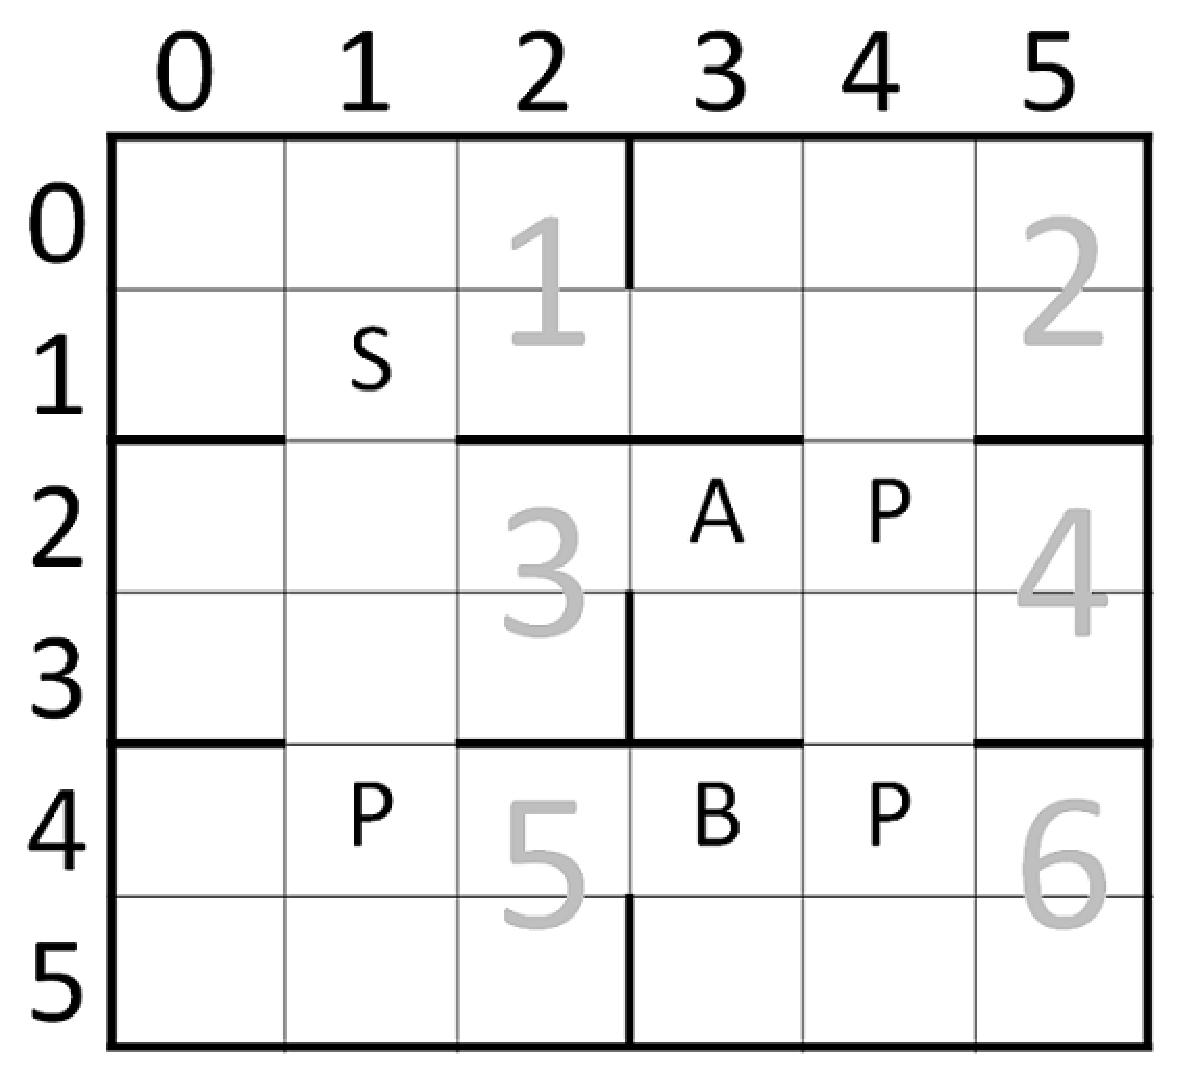
\includegraphics[width=2.0in] {./figures/BusSmall.eps}
\end{center}
\end{minipage}
\begin{minipage}[b]{0.5\linewidth}
    \begin{center}
    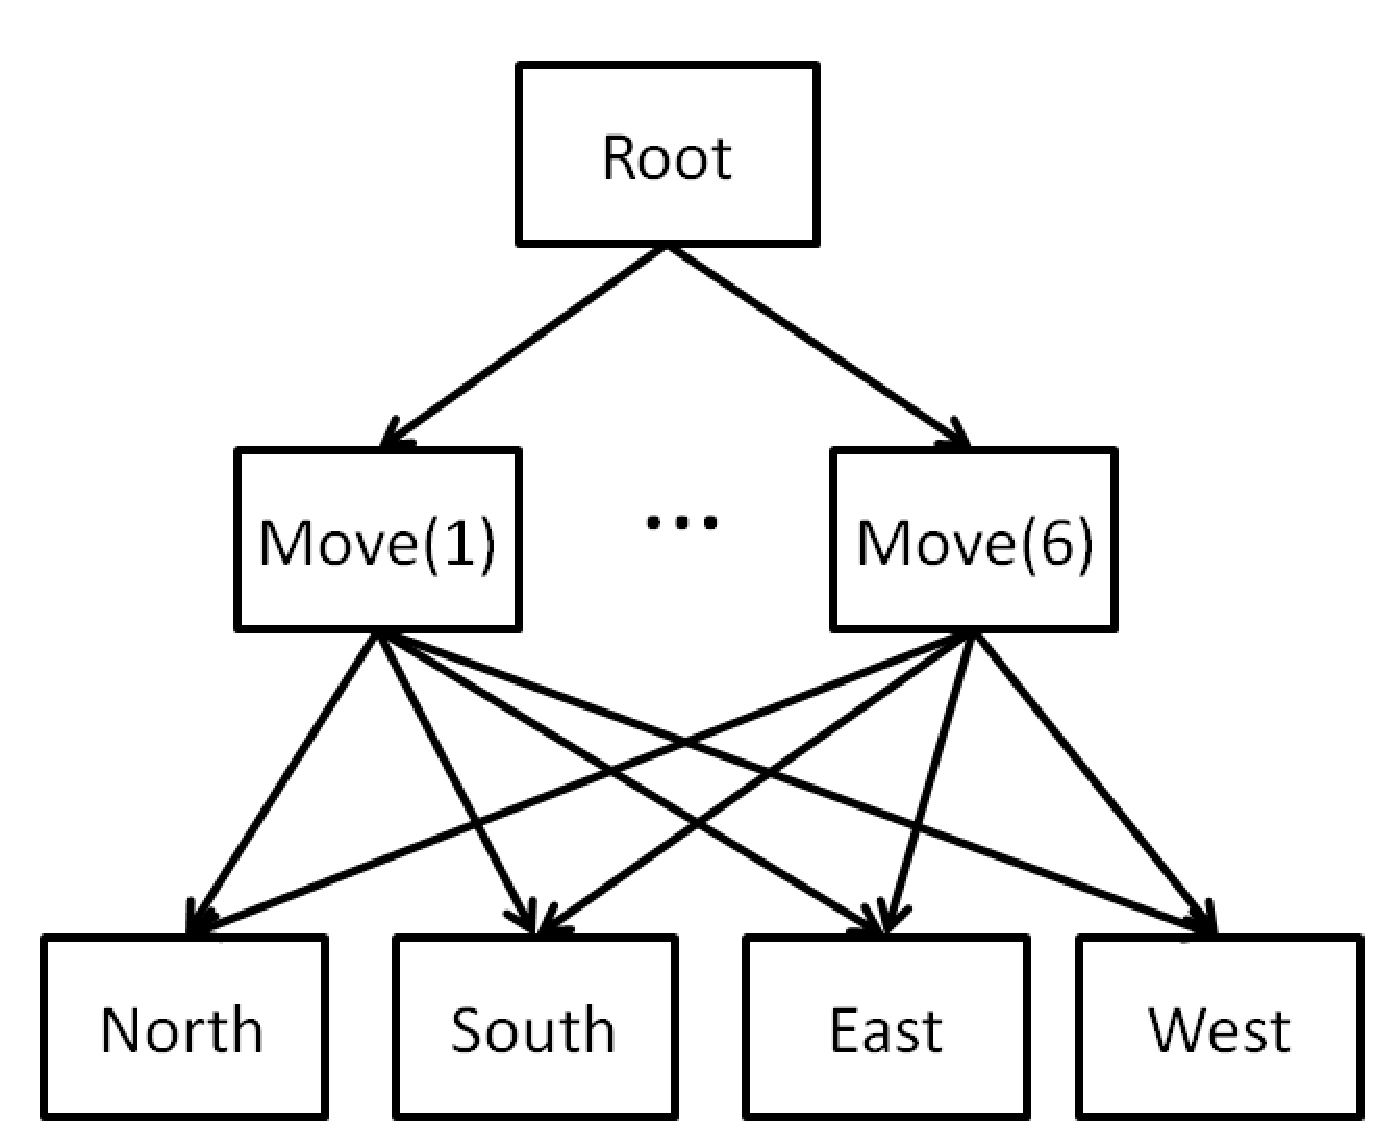
\includegraphics[width=2.0in] {./figures/BusHierarchy.eps}
\end{center}
\end{minipage}
\begin{minipage}[b]{0.5\linewidth} \centering (a) \end{minipage}
\begin{minipage}[b]{0.5\linewidth} \centering (b) \end{minipage}

\caption{(a) The Bus domain (b) A task graph for the Bus domain.}
\label{fig:bus}
\end{figure}

Figure \ref{fig:bus}(a) shows the bus domain. The bus starts at $S$. Its task
is to pickup all passengers marked as $P$ and return to $S$.
The bus can move North, South, East, or West. There is a reward of -1 applied for each action.
There is a $0.1$ probability for the bus to move in a random direction. It stays put 
when trying to cross a wall. 
The passengers are picked up automatically when the bus moves into
the location of a passenger. The passengers can be picked up in any order.
The episode ends when it finishes the task.  
There are two possible locations for road construction. They are marked as 
$A$ and $B$. If the bus passes a construction site, it will get damaged with probability 1 and has the probability
of 0.25 of breaking down for each step afterwards. There is a reward of $-50$ if the bus breaks down and the episode ends immediately. 
At the beginning of an episode, the status of the road is randomly chosen from no construction, $A$ is under construction,
or $B$ is under construction. There is a $0.05$ probability for the road status to change for each step.
The world is divided into six areas. There are six subtasks $Move(1), \dots,$ and $Move(6)$ which move the
bus to the corresponding area.
Subtask $Move(t)$ can only be invoked if $t$ is the adjacent area.
The subtask terminates if the bus exits the current area.
When it terminates, a pseudo-reward is applied if the bus arrives at designated area $t$ and 0 otherwise.
The task hierarchy is shown in Figure \ref{fig:bus}(b). 

A state can be described by a 8-tuple $(x, y, h, p_1, p_2, p_3, a, b)$, where $(x, y)$ is the location of the bus, $h$ shows if the bus is damaged, $p_i$ indicates if the corresponding passenger has been picked up or not,
and $a$ and $b$ are binary variables which indicate the status of the construction sites.

%TODO: the damage status is not perceived on the screen, so it cannot be modeled
Since the six subtasks $Move(1), \dots,$ and $Move(6)$ cover all primitive actions, they form a total leaf cover of the hierarchy.
We used HORDQ in the subtasks to guarantee the convergence to the optimal
policy. Subtask $Root$ adopted our approximate model-based method. 

%The planning variables include 
%the location of bus and the status of passengers. The environment variables are the 
%damage status of bus and the status of road. 
%TODO: total leaf cover always exist
%The world is divided by 6 areas. 

\subsection{Planning with static assumptions}
\label{se:Model}

%We adopted model-based approach 

%TODO: dyanmic programming
%TODO: add free + free HORDQ to show that HORDQ makes the hierarchical process useless
The variables of our model are $\{x, y, p_1, p_2, p_3\}$, while the damage
status and road conditions are assumed to be static during the planning process.
Our model can learn that a large penalty will be received when the bus is damaged.  
However, our model cannot learn that the bus will get damaged if it passes through
a construction site. The model is certainly biased in this case, thus
it cannot learn the optimal policy. The objective of 
the experiment is to show that the optimal policy can still be learned
if we combine the model-based approach with HORDQ. 

%Based on the results of the previous section, we can safely use any approximate model-based method 
%to learn the Q-values of subtasks which do not belong to $TC(H)$ without worrying
%that it will violate the optimality condition. Model-based RL requires the enumeration of all possible states during the planning process.
%However, it is not feasible when the state space is too large.
%Previous methods (\cite{ApproxDyna, ApproxTree}) rely on function approximation
%techniques to predict the next state. Their model is biased because it is possible 
%to encounter different next states given the same state and policy for a stochastic problem. If we 
%predict one of them, we ignore the stochastic nature of the problem. If we predict
%several, the number of states under consideration may grow exponentially with the number of simulating steps
%and become intractable after a few steps.

%We notice that, for some applications, there are some variables which are more important
%than others. Take the mobile robot navigation problem, for example; the location of the robot 
%is the key to the planning process, while the movement of other objects in the environment is less important.
%Our idea is to separate the variables into planning variables 
%and environment variables. During the planning process, we enumerate all possible values of the planning variables, while assuming 
%the remaining environment variables are static throughout the process. 
%If we limit the number of planning variables to be small, the enumeration process can be efficient.
%It also simplifies the learning of the transition and reward functions, since we only need to learn
%the dynamics and reward models for the planning variables.

Let state $s = (x, y)$, where $x$ consists of planning variables and $y$ consists of environment
variables. Following the MAXQ approach, we decompose the Q-function as:
\begin{equation}
    Q^{\pi}(i, x, j) = Q_r^{\pi}(i, x, j) + Q_c^{\pi}(i, x, j),
    \label{eq:biasedMaxQ}
\end{equation}
where $Q_r^{\pi}(i, x, j)$ is provided by the child subtask $M_j$.

The task of subtask $M_i$ is to compute $Q_c^{\pi}(i, x, j)$ by:
\begin{equation}
    Q_c^{\pi}(i, x, j) = \sum_{x'} P_m^{\pi}(x'|s, j)[Q_r^{\pi}(i, x', \pi_i(x')) + Q_c^{\pi}(i, x', \pi_i(x'))],
    \label{eq:biasedQc}
\end{equation}

With the formula above, the Q-values can be computed by dynamic programming.

For simplicity, we use the multi-time model \cite{SMDP} to model the transition function: 
\begin{equation}
    P_m(x|s, j) = \sum^{\infty}_{N=1} \gamma^N P(x, N|s, j).
    \label{eq:multiProb}
\end{equation}

$P_m(x|s, j)$ can be estimated by:
\begin{equation}
    \tilde{P}_m(x|s, j) = (1-\alpha)\tilde{P}_m(x|s, j) + \alpha [ \gamma^N \delta_{x'x}],
    \label{eq:approxP}
\end{equation}
for all $x \in S_i$, where $\delta_{x'x}=1$ if $x' = x$ and is 0 otherwise.

\subsection{Empirical results in the Bus domain}
\label{se:BusRes}
Figure \ref{fig:res}(a) shows the learning curves with different levels of pseudo-rewards.
With pseudo-reward $+60$, it learned a suboptimal policy because
the pseudo-reward is too large to make subtask $Move(t)$ ignore 
the penalty of breakdown. As a result, the subtask followed 
the instruction of its parent too strictly.

On the other hand, if we do not impose any pseudo-reward, 
the optimal policy can be learned, but the learning rate is
slower than SARSA(0) learning. Since subtask $Move(t)$ has no
incentive to follow the instruction of its parent subtask, 
the learning process is similar to SARSA(0) learning 
except it has six different Q-functions to learn (one for each subtask) instead of one.
Thus it takes longer to learn the optimal policy. 

With an appropriate pseudo-reward, we can get a near-optimal policy
while the learning rate is faster than SARSA(0).
Our experiment shows that a pseudo-reward of +5 is enough to make subtask $Move(t)$ follow 
the order of $Root$ in most of the times, but it is not enough for the subtask to ignore
the breakdown penalty. For example, when $Root$ executes $Move(4)$ to move the bus from area 
3 to area 4 and the road at location $A$ is under construction, $Move(4)$ subtask
will learn it is a bad decision with HORDQ.
Instead of moving to area 4, $Move(4)$ may move to area 1 or 5 to avoid
the breakdown penalty. In turn, $Root$ learns that $Move(4)$ cannot be executed in 
such a scenario, thus it will seek an alternative plan if the same scenario
is encountered.

To illustrate the undesirable result when some suboptimal subtasks exist in 
the hierarchy and the MAXQ framework is adopted, we combine our approximate model-based approach
and MAXQ-Q learning in our experiment. The combination learns a suboptimal policy similar to HORDQ with high pseudo-reward. 
Since MAXQ does not estimate the consequence of its action outside its own subtask,
$Move(t)$ will move to area $t$ at any cost. It leads to the frequent damage of the bus.

To simulate the performance of the combination of a poorly-approximated model-based method and 
HORDQ, we replaced our model-based approach with a random policy.
The result is shown in Figure \ref{fig:res}(b). In this case, SARSA(0) has the fastest
learning rate. It takes more time for $Move(t)$ to realize that the policy of $Root$ is bad with higher pseudo rewards.
Nevertheless, it will eventually learn a near-optimal policy.
The combination of random policy and MAXQ presented the worst result.

This result shows that a good approximate model 
can help increase the learning rate with the combination of HORDQ. 
If the model is poor, HORDQ serves as a fail-safe mechanism to keep 
the agent from repeating the same poor policy over and over again.
On the other hand, MAXQ learned a poor policy in both cases.  
This evidence suggests that in order to construct a robust HRL 
algorithm, it is beneficial to incorporate HORDQ in the hierarchy.

\begin{figure}[b]
%\begin{center}
 \begin{minipage}[b]{0.9\linewidth}
     \begin{center}
    %\includegraphics[height=11em, width=6em]{eli_bend.eps}
    \includegraphics[width=3.5in] {./figures/Approx.eps}
\end{center}
    %\caption{(a)}
\end{minipage}
\begin{minipage}[b]{0.9\linewidth} \centering (a) \end{minipage}
\begin{minipage}[b]{0.9\linewidth}
     \begin{center}
    \includegraphics[width=3.5in] {./figures/Random.eps}
\end{center}
\end{minipage}
\begin{minipage}[b]{0.9\linewidth} \centering (b) \end{minipage}
%\end{center}
\caption{The learning curve for the bus domain, averaged over 400 episodes. (a) With our model-based approach. (b) With random policy.
The pseudo-reward is shown in parentheses. The parameters are $\alpha=0.1$ and $\gamma=1$. All algorithms follow an $\epsilon$-greedy exploration policy
with $\epsilon = 0.1$.}
\label{fig:res}
\end{figure}


\vfill
\clearpage

%\newpage
%TODO:
%The above experiment assumes the agent knows when
%it will receive the delayed reward.
%However, it 
%It is not a p

%On the contrary, the combination of MAXQ and a poor approximated model has
%a performance similar to random policy.

%TODO: add random agent experiment
%TODO: if I set the pseudo reward to zero, will the whole stuff breaks down again?


\section{Infinite Mario}
\label{se:MarioExp}
%reward system here
%and pseudo reward
We use Infinite Mario to show the effectiveness of our approach in large domains. 
Large domains contain more than millions of states, so it makes table-lookup methods not applicable
due to the curse of dimensionality. Approximation techniques are required to handle these
problems, but the optimality guarantee will be lost.
It is interesting to see how our work will perform with function approximation techniques,
especially when model-free methods cannot learn the optimal policy.

\subsection{Previous work}
Infinite Mario is an open source Java implementation of Nintendo's Super Mario Brothers game.
It received much attention in the AI community possibly due to
the two AI competitions -- RL 2009 competition\footnote{http://2009.rl-competition.org/}
and Mario AI competition\footnote{http://julian.togelius.com/mariocompetition2009/}, which were held in 2009.
The objective of these competitions is to build the best agent that
can play this classic side-scrolling arcade-style game.

%Bruno In the paragraph above, perhaps you could cite the competitions, at least as a footnote directing to their web site
%James added

The RL 2009 competition required competitors to use RL algorithms to build their agents.
On the other hand, the Mario AI 2009 competition \cite{Robin09} 
did not pose any restrictions on the underlying technique.
It encouraged
competitors to use neural networks, genetic genetic programming, fuzzy logic, temporal difference learning, and human ingenuity.

The observation of Mario AI in RL 2009 competition 
contains the location and speed of Mario and other monsters, as well as
the $22 \times 16$ tiles on the screen.
The agent receives +100 reward when it finishes a level, +1 reward when collects
a coin, and -10 reward when it dies.

%Since this competition focuses on RL algorithms,
%the agent needs to learn the property of environment through interaction.

Mohan and Laird \cite{Mohan09} combined HRL and Soar-RL \cite{Nason05} to build
a Mario agent. In their hierarchy, the task is divided to "Grab Coin", "Search Question", "Tackle Monster",
"Avoid Pit", and "Move to Goal". 
The root subtask chooses one of these subtasks to execute based on the learned
preferences. Each subtask deals with at most one object. For example, the
"Grab Coin" subtask is considered successful only when the specified 
coin is collected. Thus, the number of subtasks available for the root task to choose
depends on the current objects in the screen.

Gibson and Risk \cite{Gibson09} adopts the options framework.
The master agent can execute 3 options -- a $SARSA(\lambda)$ agent, a "pit specialist" agent, and a
rule-based agent. The "pit specialist" concerns only with the pits, and is available only when
there is a pit within 4 tiles of Mario. 
The master agent uses SMDP Q-learning to learn which option to execute given a state.

Ringstad et al. \cite{Paul09} 
used a modified linear SARSA algorithm to build the agent.
The input features are the locations of the 3 nearest monsters or pits.
Their idea is to design an agent that can finish the level as fast as possible.
To encourage the agent to finish the level, they rewarded the agent when it traverses
intervals of 10 tiles away from the start.
Their method won the Mario AI championship of RL competition 2009.

%Bruno What is a pseudo-reward? And shouldn't you be describing these contributions in the related work section of your thesis? Possibly in a separate chapter?
%James The reference of pseudo-reward has been removed.
%James It is good question. My concern is that the related work presented here is only related to Mario experiment. Where should I put it?

The state observation of Mario AI 2009 competition \cite{Robin09} includes $22 \times 22$ tiles on the screen, the location and the speed of monsters, 
and the status of Mario such as "isMarioOnGround" or "mayMarioJump".

%Bruno What do these status variables have in common? Are there others? How many variables are there? What's the # of dimensions in the state?

%Booleans: mario is on the ground, may
%jump, is carrying a shell, is small/big/fireprovides an interface
The techniques which are adopted by the competitors of Mario AI competition include
$A^*$ search, genetic programming, hand-coded policy, a hybrid method of neural network and $A^*$ search,
and Cyberneurons.
In general, $A^*$ search achieves the best result, and hand-coded policy falls the second.
Robin Baumgarten \cite{Robin09} won the championship of the Mario AI competition in 2009.
His idea is to create a physics engine that can accurately predict the next state of Mario, 
and use $A^*$ search to find a path to the right border of the screen as fast as possible.
Since his approach requires the agent to have the complete knowledge of the environment,
the approach falls into the category of classical planning.

%Bruno So if classical planning won the competition, either the learning agents were really bad (therefore a bad baseline)
%or the domain is not challenging enough right?
%James Because the classical planning has the complete knowledge of the problem, but RL methods do not.
%James You may that say the domain is not challenging, since we do have the complete knowledge of Mario, but it may not be true for other video games.

Ross et al. \cite{Ross11} used supervised learning to learn the direct policy
mapping between input features and the primitive actions. The input features
are $22 \times 22$ tiles around Mario in previous 4 frames, the state of Mario
and the last 6 actions. The tiles include the types of the ground, blocks, and
monsters.  The state of Mario includes the types (small, big and fire Mario) as well as a
binary feature to indicate if Mario touches the ground or not.
The training data is obtained through search-based methods similar to Baumgarten's work \cite{Robin09}.


The above approaches either depend on game-specific information ("isMarioOnGround")
or depend on the information that is difficult to be retrieved from image features (the location and size of pits).
In this section, we introduce an approach 
of building an agent for Infinite Mario 
without using such information.
We only restrict the agent to use the features provided by the simulator of Infinite Mario from RL competition 2009.
The features can be retrieved from the screen directly, 
therefore it allow us to generalize our approach to other video games without
the need to redesign specialized features for each individual problem.

%Our goal
%is to train the computer to play this game based on the current
%game image features as input (see Figure 3).

%why RL competion is pure image based
%We do not reguire the agent to have prior knowledge about some special tile patterns which are game-specific

%to allow the agent to simulate its own action in the environment that is identical
%to the game itself. It allows people to use the techniques in classical planning,
%such as search-based methods. 

%Infinite Mario, a Java implementation of Nintendo's Super Mario Bros. game, becomes
%a recent interest in the AI community.
%There is also a recent interest in developing agents that can play a complete side-scrolling
%arcade-style game. In 2009, two AI competitions were organized on agents that can play
%entire levels of Inite Mario, a clone of Nintendo's popular Super Mario Bros game. The
%RL 2009 Competition [Mohan and Laird, 2009] requires the agents to use reinforcement
%learning to learn to play the game. The learning agents are given a state representation
%containing the location of the player character (PC) and other monsters, as well as the types
%of the individual tiles on the screen. The agents receive a positive reward once the level is
%complete, and a small negative reward on all other states. The Mario AI Competition4, on
%the other hand, does not limit the agents to a speci approach. Indeed, the participants
%are encouraged to use evolutionary neural networks, genetic programming, fuzzy logic,
%temporal dirence learning, human ingenuity, [and] hybrids of the above"5. Playing an
%Atari 2600 game was previously attempted by Diuk et. al., who illustrated the performance
%of their Object-Oriented Rmax algorithm by teaching the Player Character to pass the st
%screen of the game Pitfall [Diuk et al., 2008].
%A shared characteristic between all the above examples, and (to our knowledge) all
%previous attempts of learning to play video games, is that each agent is designed and tuned
%to play a single game. Therefore, all the essential game properties (e.g., the location of the
%PC and important NPC's, health levels, and timers) are either explicitly included in the
%state representation, or can be easily extracted form it. Also, game-speci abstractions are
%often performed to deal with the large state-space. Furthermore, the reward signal may be
%shaped in a way to accelerate the learning.
%One of the key distinctions of the methods described in this thesis is their generic nature.

%Screen feature
%assume the location of PC is known
%the result is unknown (the properties of monsters or coins)

\subsection{Infinite Mario domain}

We use the 2009 RL competition environment to conduct our experiment.
The action space of Infinite Mario consists of 4 buttons which correspond
to the original Nintendo controller.
These buttons are:
\begin{itemize}
%\item Handle the interaction between objects
%\item Not everything can be modeled
\item Direction pad: left or right
\item A button: jump
\item B button: speed
\end{itemize}
Mario can choose to press these buttons or not, so
the number of possible actions are $3 \times 2 \times 2 = 12$ actions.  

We exclude action "speed", "jump speed" and "no op" from the 
action space, since they do not seem to be relevant to the optimal policy.
The agent can execute 9 actions in our experiment.

%Bruno At this point you could say already if something belongs to the optimal policy or not, since you claim that your method learns this policy right?
%James In Mario domain, it is not clear what the optimal policy is, due to the huge state space.
%James Do you suggest me rephrase it?

The screen of Infinite Mario is comprised of a matrix of $22 \times 16$ tiles.
The matrix is an array of characters, with each element representing the type of tile.
The types of tile are brick, question-block, coin, pipe, empty tile, the finish line and Mario.

Besides the tile information, the information of moving objects are also provided. 
The moving objects are Mario, Red Koopa, Green Koopa, Goomba, Spikey, Piranha Plant, Mushroom, Shell, Fire Flower and Fireball.
The information of each object includes x- and y-positions, x- and y-velocities, and type of object.
Note that the positions and velocities are continuous, so a quantization technique might be required.

The tile information can be captured from screen with basic image processing techniques \cite{Yavar}.
The location and speed of monsters can be obtained by applying computer vision techniques such
as object tracking or optical flow.

The levels are generated with 3 parameters: random seed, type, and difficulty.
The difficulty ranges from 0 (easiest) to 9 (hardest). 

The agent will receive the following rewards:
\begin{itemize}
%\item Handle the interaction between objects
%\item Not everything can be modeled
\item +100: finishing a level
\item +1: collecting a coin
\item +1 : hitting a question block
\item +1 : killing a monster
\item -0.01 : step cost
\item -50 : getting killed
\end{itemize}

Besides, we apply a reward equal to the
displacement of x-position to encourage the agent to move as right as possible
and penalize the agent if it moves to left.

%Bruno Where this choice come from? Would your method work without it?
%James Because Mario doesn't know the exit is at the far end of his right, it needs some motivation to move in that direction.
%James So no method will work without it.

\subsection{The model-based method for Mario domain}
%TODO: only 9 actions
%TODO: sampling

\begin{figure}[t]
 \begin{minipage}[b]{0.45\linewidth}
    \begin{center}
    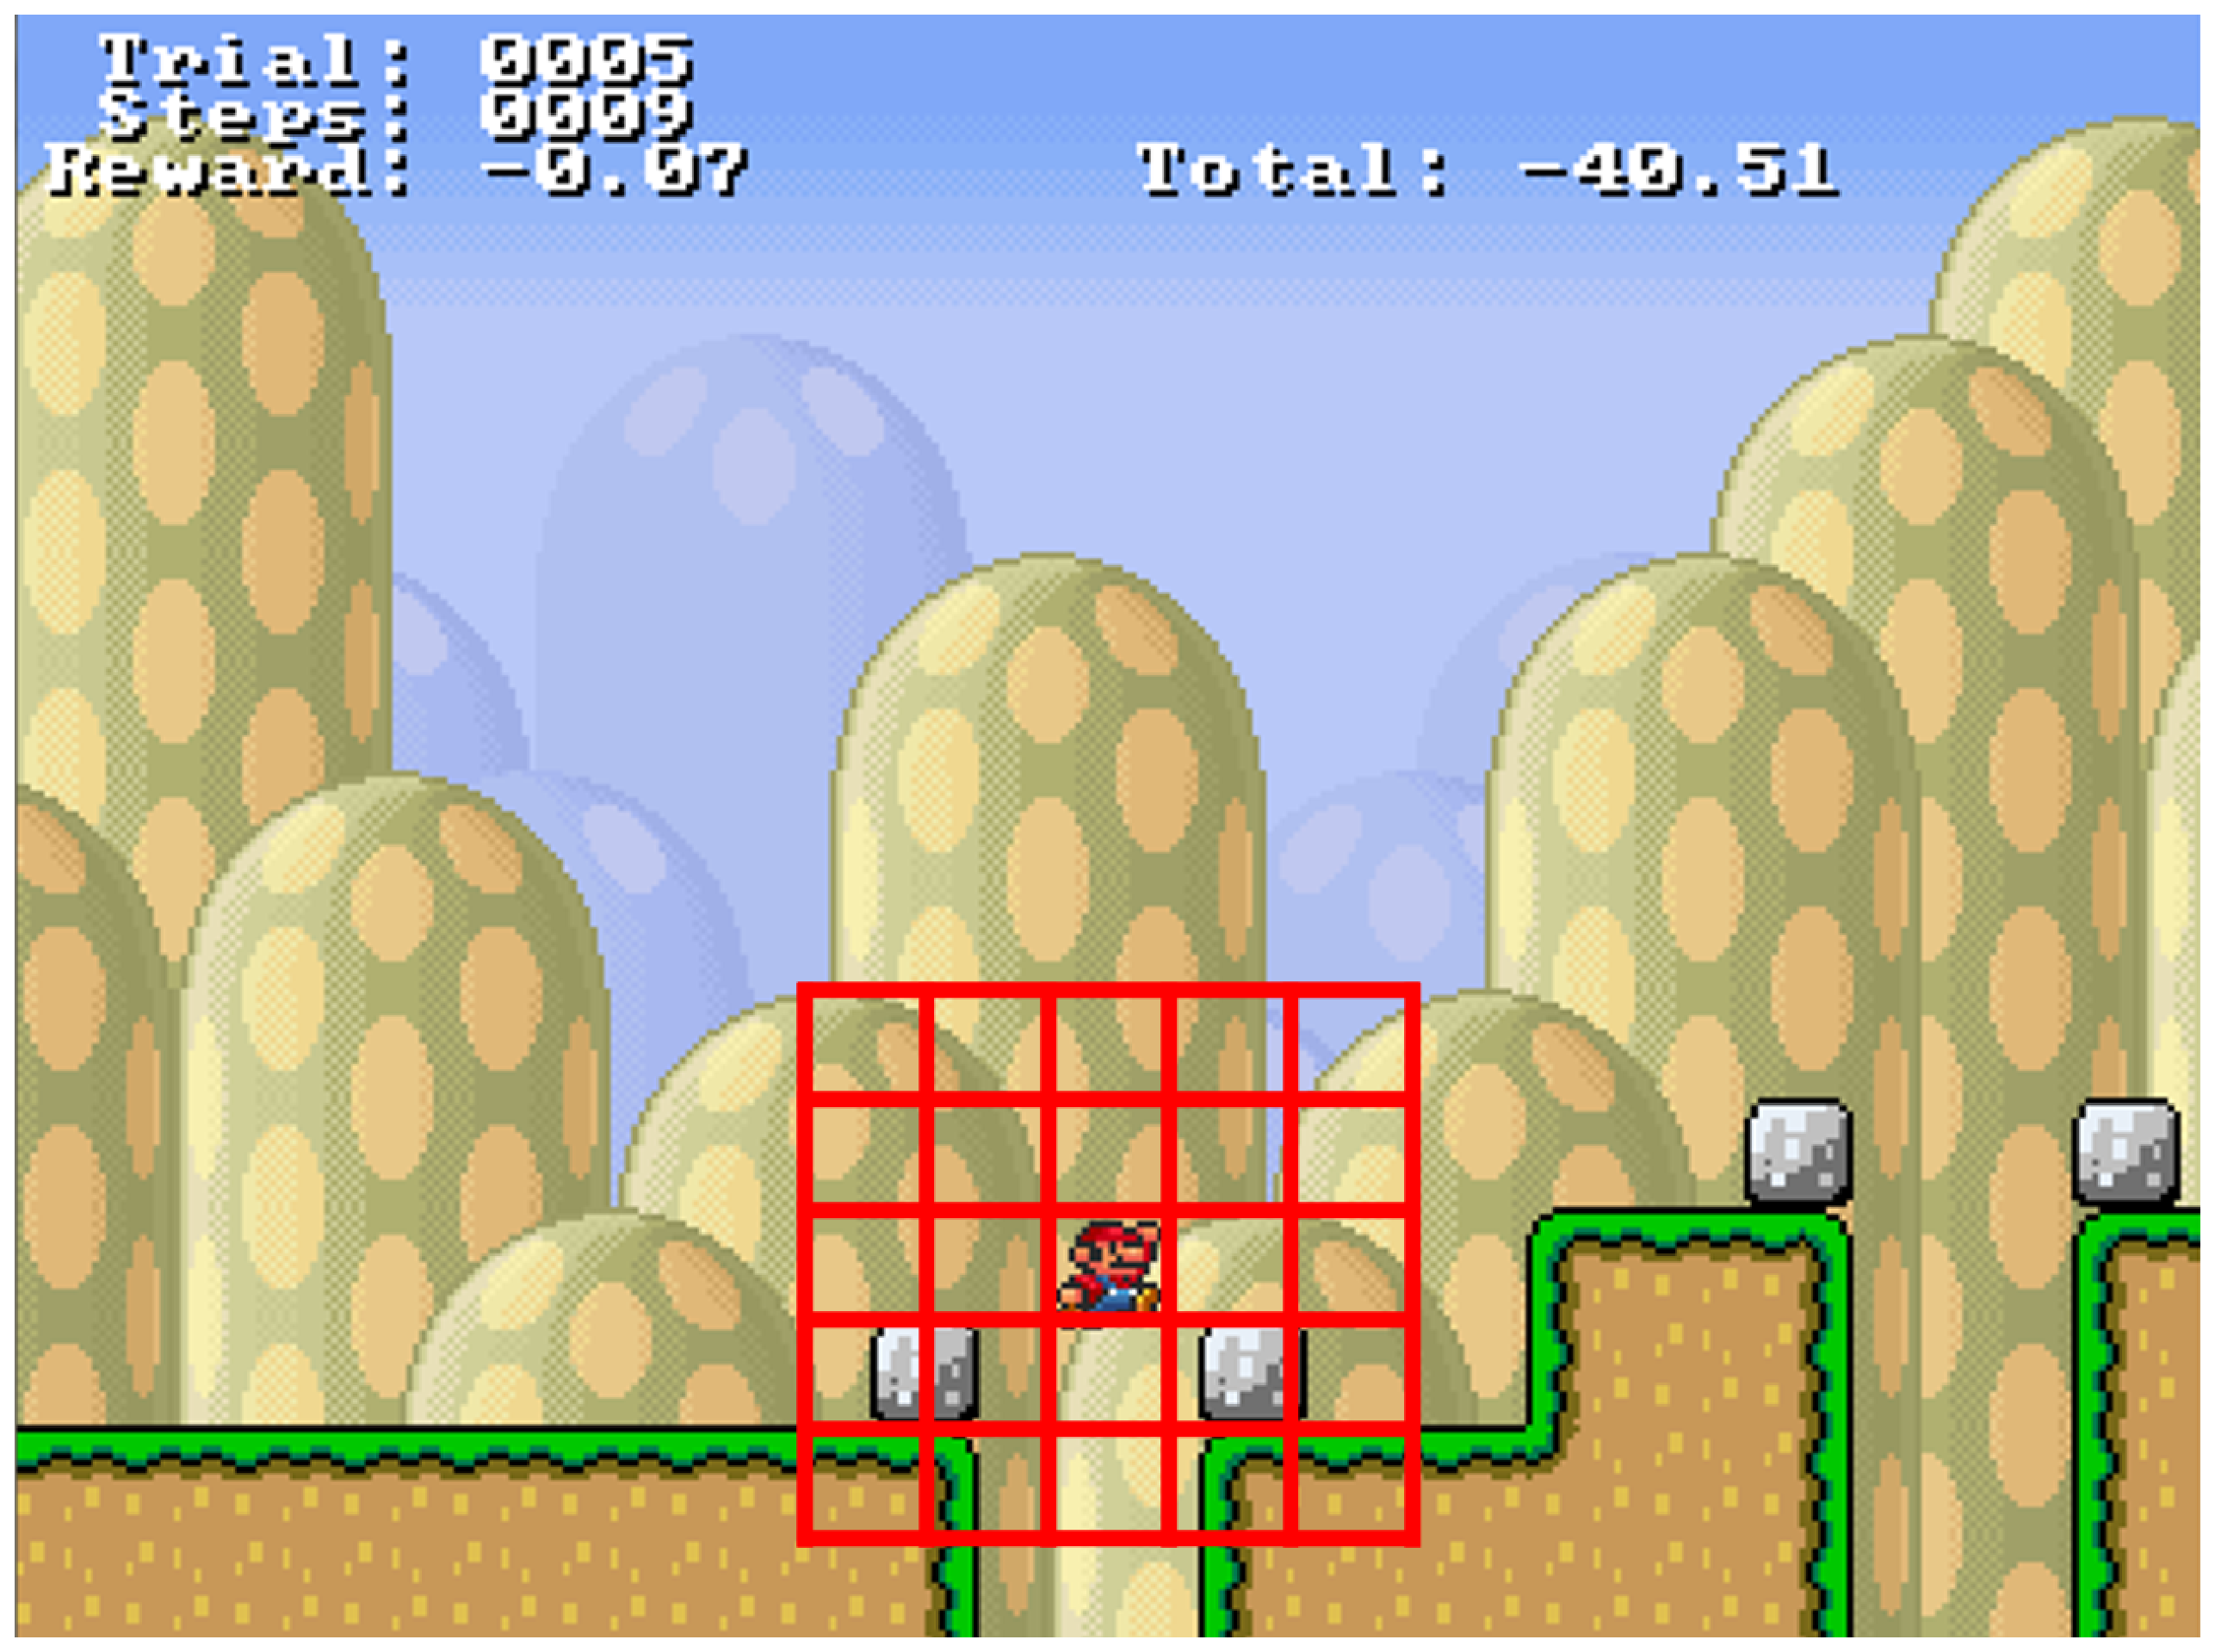
\includegraphics[width=2.0in] {./figures/MarioGrid.eps}
\end{center}
\end{minipage}
\begin{minipage}[b]{0.45\linewidth}
    \begin{center}
    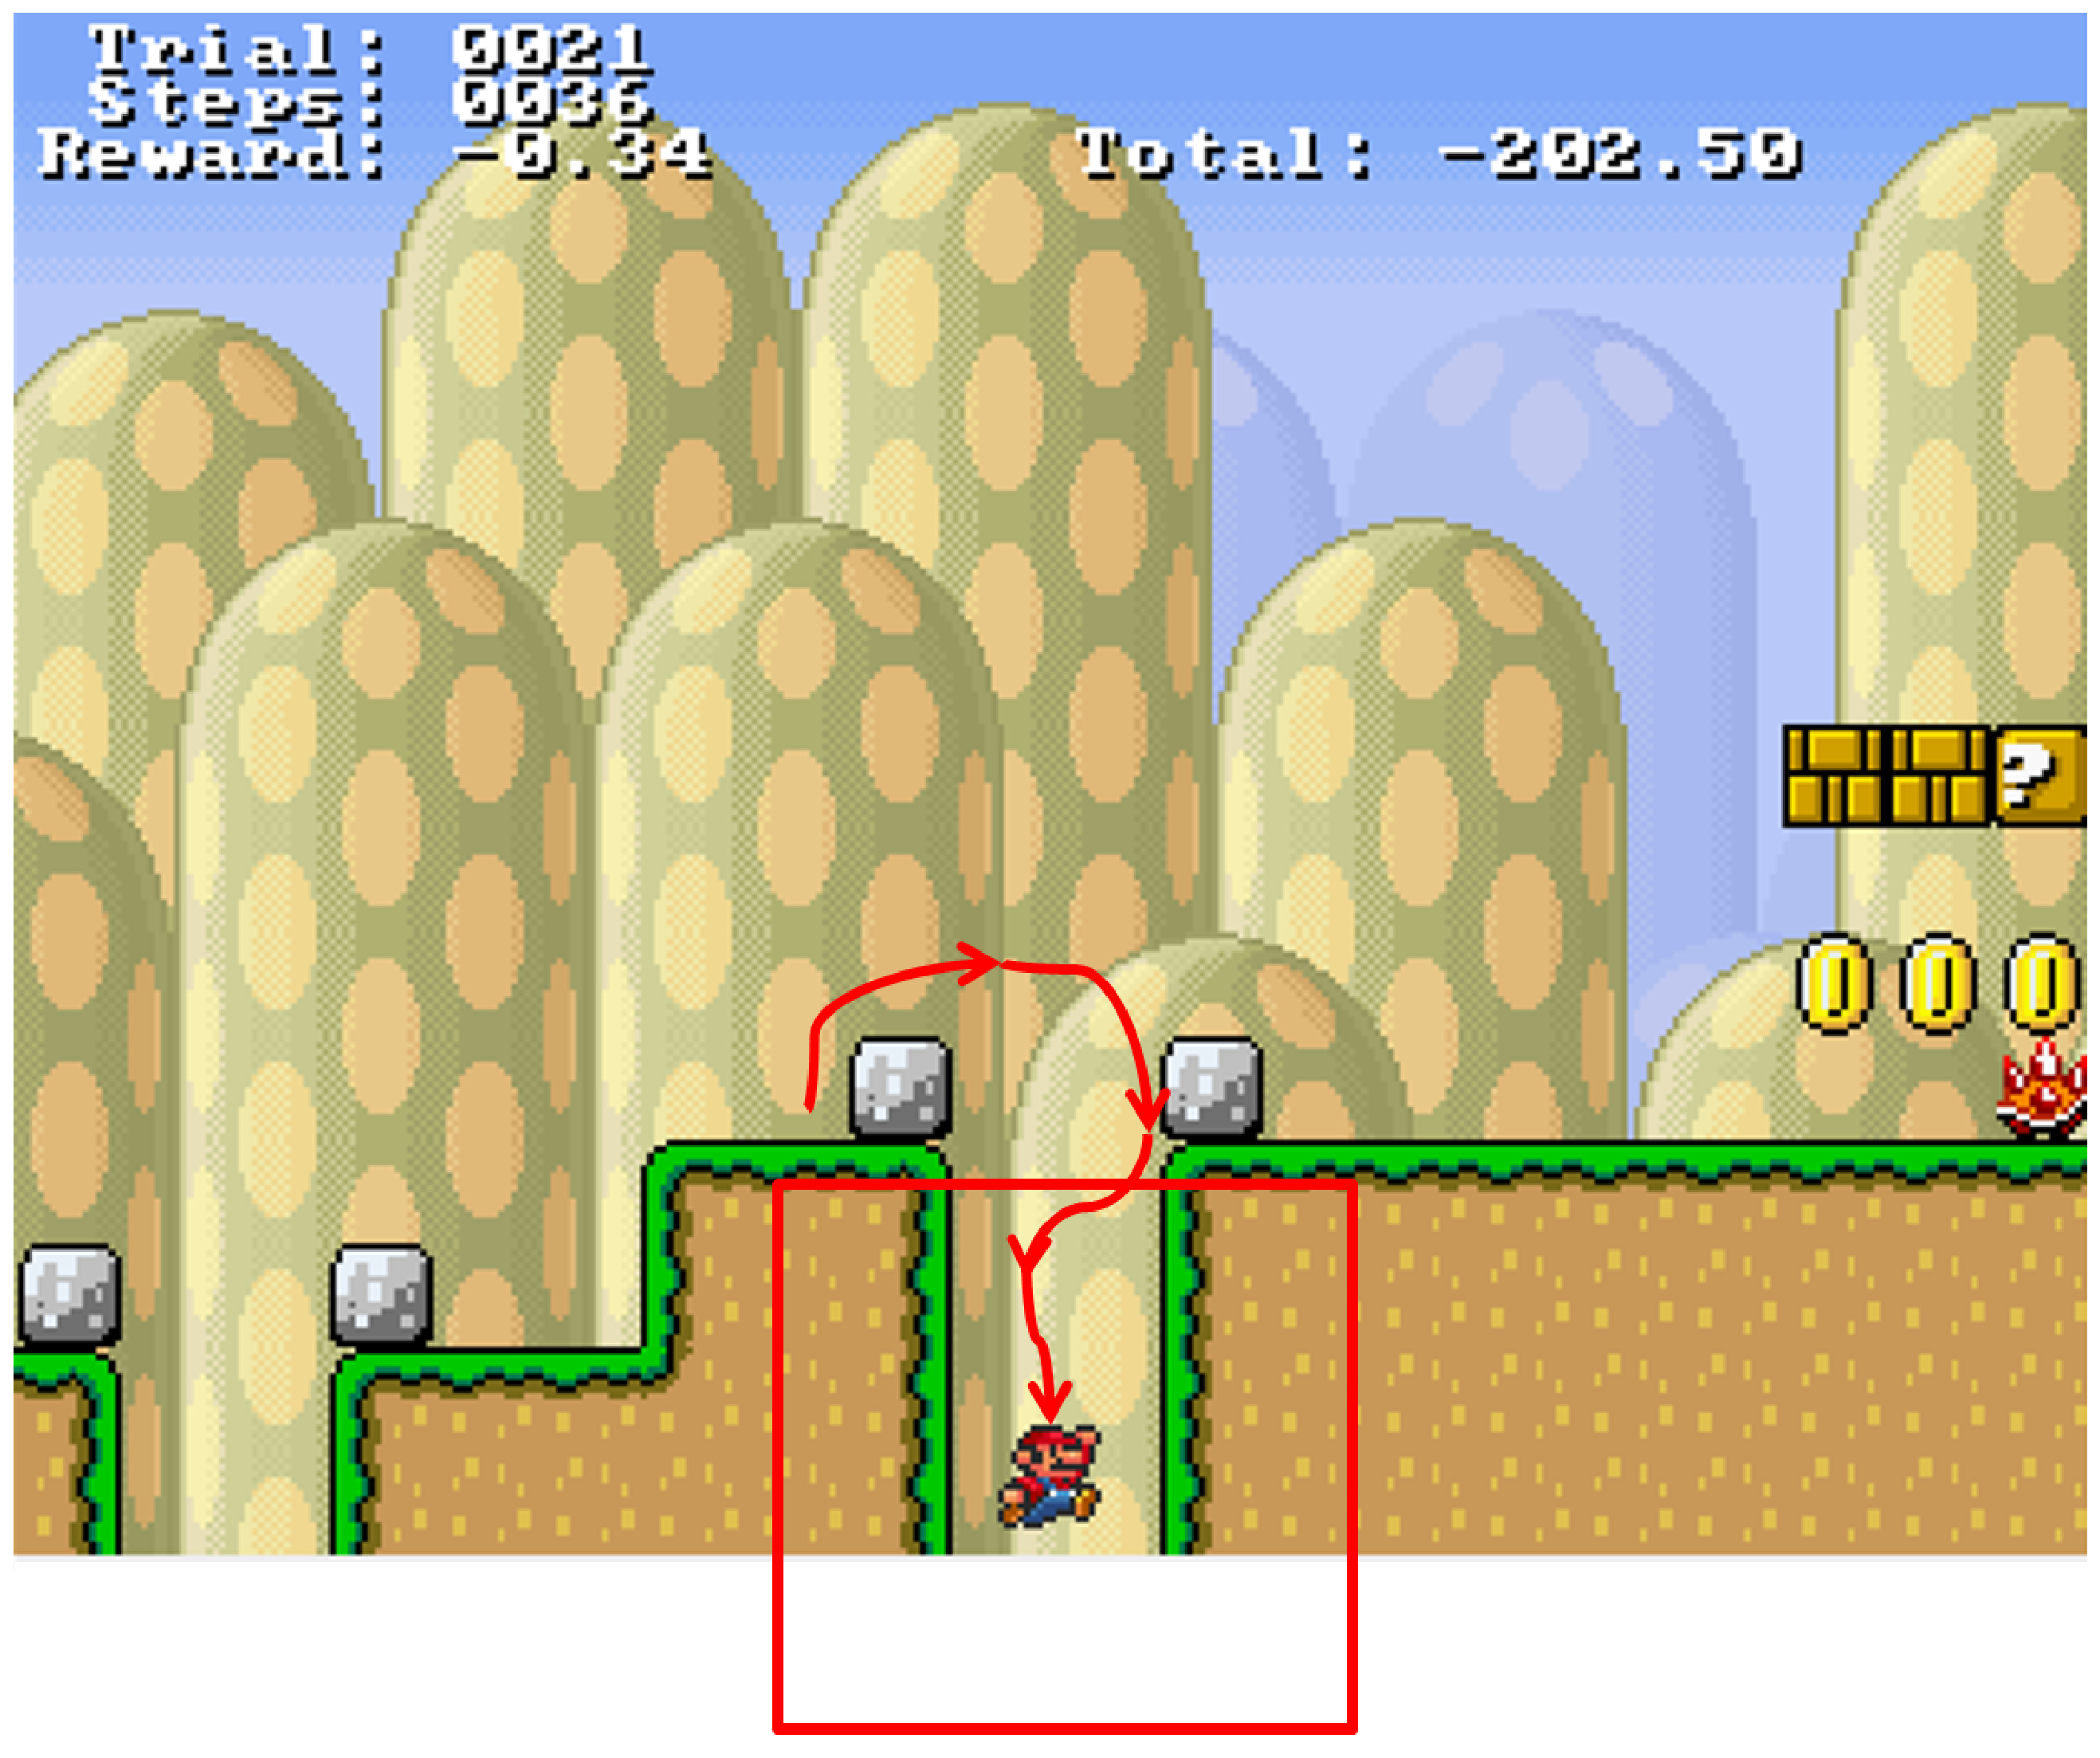
\includegraphics[width=2.0in] {./figures/MarioModel.eps}
\end{center}
\end{minipage}
\begin{minipage}[b]{0.45\linewidth} \centering (a) \end{minipage}
\begin{minipage}[b]{0.45\linewidth} \centering (b) \end{minipage}

\caption{(a) A screenshot of Infinite Mario (b) A planning process conducted by the search-based method.}
\label{fig:Mario}
\end{figure}

%We adopt greedy search in our planning process.
%The planning process begins with a state of Mario. 
%Then it iteratively acquires the next states by applying
%the 9 actions to the state. To avoid fully expand the whole search tree to 
%the depth $K$, which is time-consuming and unnecessary, we expand the state

We adopt the model-based method to learn the transition function of Mario.
The state of Mario 
can be described by a 4-tuple $(x, y, dx, dy)$, where are the location and velocities of Mario. 
The ranges of $x$, $y$, $dx$ and $dy$ are $[0, 318]$, $[0, 15]$, $[-2.5, 2.5]$, and $[-2.5, 2.5]$.
These variable are continuous, so it is not possible to enumerate all possible states
of Mario with dynamic programming techniques. It is possible to discretize the variables, but the resulting state space 
would still be too large if we want to predict the dynamics of Mario precisely.

Instead of discretizing the variables, we used the regression tree algorithm
in the Orange package \cite{Orange04} to predict the future position and speed of Mario.
The features are the current speed of Mario and the tiles within 5 by 5 
area around Mario (Fig. \ref{fig:Mario}(a)). There are 27 variables. 
Since each action has different dynamics, 
we build different trees for different actions. 
Given the current state and action, the regression trees should predict 
the speed and position of the following state. 
The regression trees predict
the relative changes of positions $\epsilon_x = x' - x$ and 
$\epsilon_y = y' - y$ since modeling relative change might generalize better across states \cite{Hester09}.
However, the relative changes of speeds do not generalize well, so we predict
the value of speeds directly.
%(a possible reason is that the maximum speed is capped, so Mario cannot
%keep increasing its speed by press the speed button). 
The x-position, y-position, x-speed and y-speed are the class variables for the regression trees.
For simplicity, we separately build regression trees for different class variables and actions. 
In our current implementation, there are 9 actions and 4 class variables, so we 
have 36 regression trees to model the dynamics of Mario. 

We borrowed the idea of Baumgarten \cite{Robin09}, using
the search-based method to find a sequence of actions that moves Mario to the right edge of the screen as fast as possible.
Instead of hard-coding the objective of the search process, we add a possible reward to the agent if it moves
to the right and a negative reward otherwise.
We adopt a simple k-step lookahead greedy search in our planning process.
It begins with the current state of Mario. 
Then it expands one node in the search tree by applying all possible actions. 
To avoid fully expanding the whole search tree to 
the maximum depth, which is 6 in our experiment, we use greedy search and expand the node
with the largest predicted reward. 
The process stops after the number of nodes exceeds 300, then the search algorithm returns 
a sequence of actions which achieves the highest predicted reward.
To reduce the computation time spent on searching, the search algorithm will return
immediately if there is a sequence of action which gets more than +6 reward.
There are $9^6=531,441$ nodes in the fully-expanded tree. 
Since we only search a very small part of it, it is possible for the search algorithm
to return a suboptimal sequence.
The locations of monsters and other objects are assumed to be the same
during the planning process. 

It is crucial for the search-based method to learn when Mario is going to be killed. 
However, the number of samples right before Mario gets killed is limited by the
number of episodes due to the fact that the episode terminates immediately after the death of Mario.
To efficiently use the available samples, we use a single regression tree to learn the 
reward function. The input features of the regression tree are
the features for the transition function plus the action of the agent. 

The strength of the above method is that it has the terrain knowledge and can move
efficiently to finish a level.
%Another advantage is that it can predict a sequence of actions to jump over a pit.
%The primary difficulty for model-free methods to deal with the pit is that 

%It is quite often that Mario suffers a inevitable death (such as jumps into a monster or falls into a pit).
%If such a scenario happens, there are no actions that can save Mario.
%All action sequences will have a negative predicted reward, so our early return heuristic does not work.

%all possible states of Mario, the planner in our experiment 
%is a $K$-step lookahead greedy search algorithm. The planner searches the states
%which can be reached from the current state within $K$ steps and returns a sequence of
%steps which achieve the highest reward.


%It is crucial for the planning process to learn when Mario is going to be killed. 
%However, the number of samples right before Mario getting killed is limited by the
%number of episodes, which is much smaller than the number of steps. 
%To efficiently use the available samples, we use a single regression tree to learn the 
%reward function.


%To adopt $A^*$ search
%We adopt our static assumption on all objects except Mario. 



%

%TODO: objective: generic AI, challenge here (no specific domain knowledge)
%why model-free approach is necessary

Since we only model the dynamics of Mario, effects such as the dynamics of other objects or
the interactions between objects are ignored. 

Here is the list of effects which are not included in the model:
\begin{itemize}
%\item Handle the interaction between objects
%\item Not everything can be modeled
\item Monsters may appear at the right edge of the screen
\item Monsters disappear at the left edge of the screen
\item Monsters can be killed by Mario, a fireball, or a moving shell
\item Monsters can be killed by falling into a pit
\item Koopma can be turned into a shell
\item Mario can kick a shell to make it move
\item Jump on top of a moving shell will make it stop
\item Fire Mario can attack with fireballs
\item Small Mario can be turned into Big Mario by consuming a mushroom
\item Big Mario can be turned into Fire Mario by consuming a fire flower
\item Coins, mushrooms and fire flowers can be consumed by Mario
\end{itemize}

To learn the transition function perfectly, it is necessary to 
learn all the effects correctly. However, learning the effects for a stochastic
problem is NP-Hard \cite{Walsh09} and heuristic solutions are required
to solve it \cite{Pasula07}.

Our work provides an alternative approach to this problem--instead of learning 
all possible effects, we only learn part of them and 
let model-free methods handle the scenarios associated with
the effects which are not included in the model.

The 5 by 5 tiles around Mario include the monsters as well,
so it is possible for the model-based method to learn the imminent
death caused by moving Mario directly to monsters. What it cannot handle is the delayed death cases, which happen when
Mario moves very close to monsters, but does not touch it.
In such a scenario, it doesn't matter which action Mario is going to take, 
the subsequent death is guaranteed. 
This also happens when Mario moves to a position which will be surrounded by
monsters. After Mario moves to such a position, Mario will be killed inevitably.
%Since there are no way out, the death is inevitable. 
The supervised learning can only learn the reward function with immediate reward.
When the death is actually caused by a decision made few steps before, it is difficult
for a supervised learning algorithm to figure out such a relationship. 
On the other hand, such a delayed feedback will propagate back to previous states with model-free methods
such as $SARSA(\lambda)$, so it is not a problem for these methods.
%The heuristic to reduce the search time
%TODO: up to 6 tiles away
%TODO: no jump involved when it is not going to move up (list all primitive actions, and why they greatly reduce the search space)
%TODO: stop search when is the reward to too negative

%details
%model-based approach knows both tile info and monster info



%The generality of my approach presented here
%If we have a perfect simulator which is identical to the environment, 
%it is possible to use K-step lookahead to find an path from beginning
%to the end (TODO: Mario Competition here). We do 
%conduct the planning process perfectly without 
%resort to 
%It is possible to have a pe

\subsection{The model-free method for Mario domain}

%Bruno Perhaps this section could be called The model-free method and its relation to the problem you illustrated before.
%James Title changed

Since the model-based method cannot deal with the interaction between objects, we use a
model-free method to handle it.

The features of model-free methods include the types and locations of moving objects
other than Mario itself. To reduce the number of features, we do not include the speed of objects.
As noted in \cite{Gibson09}, it is more generalizable if we use "egocentric representation".
That is, we use the relative positions between Mario and objects 
as the features instead of the absolute positions.

Since the number of monsters can be any arbitrary number, 
we cannot use linear SARSA which depends on a fixed feature size.
Instead, we use relational approaches here. 
We incorporated relational temporal difference learning (RTDL) \cite{RRLTD}
with HORDQ. RTDL is a relational extension to linear SARSA, thus it does not
work for continuous variables. To discretize them, we simply
round each variable to the nearest integer. 

Unlike previous approaches \cite{Paul09, Gibson09, Mohan09, Mohan10},
we do not include the location of pits in our features.
Since the pit is not a moving object nor does it occupy a single tile,
it is not available in the input features.
Previous approaches relied on prior knowledge of the shape and size of pits to parse the tile information
and extract the location of a pit. 
We argue that this would not contribute to the generality of the method.
It would be possible to include the pit information by using the whole screen ($22 \times 16$)
as the feature. But the potential huge state space makes it inapplicable in practice ($14^{352}$ states with 14 different types of tiles)
Moreover, it is not necessary to include the pit information in model-free methods,
since the pit can be handled by the model-based method. 

\subsection{The hybrid approach}
\begin{figure}[ht]
 %\begin{minipage}[b]{1.0\linewidth}
    %\begin{center}
    %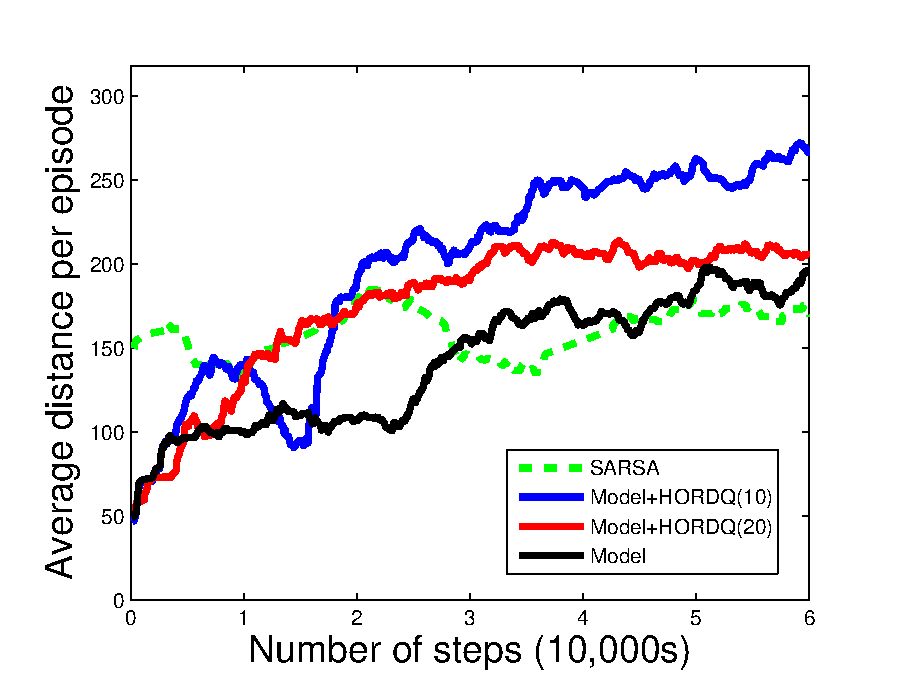
\includegraphics[width=4.0in] {./figures/1247.eps}
%\end{center}
%\end{minipage}
%\begin{minipage}[b]{0.5\linewidth}
    \begin{center}
    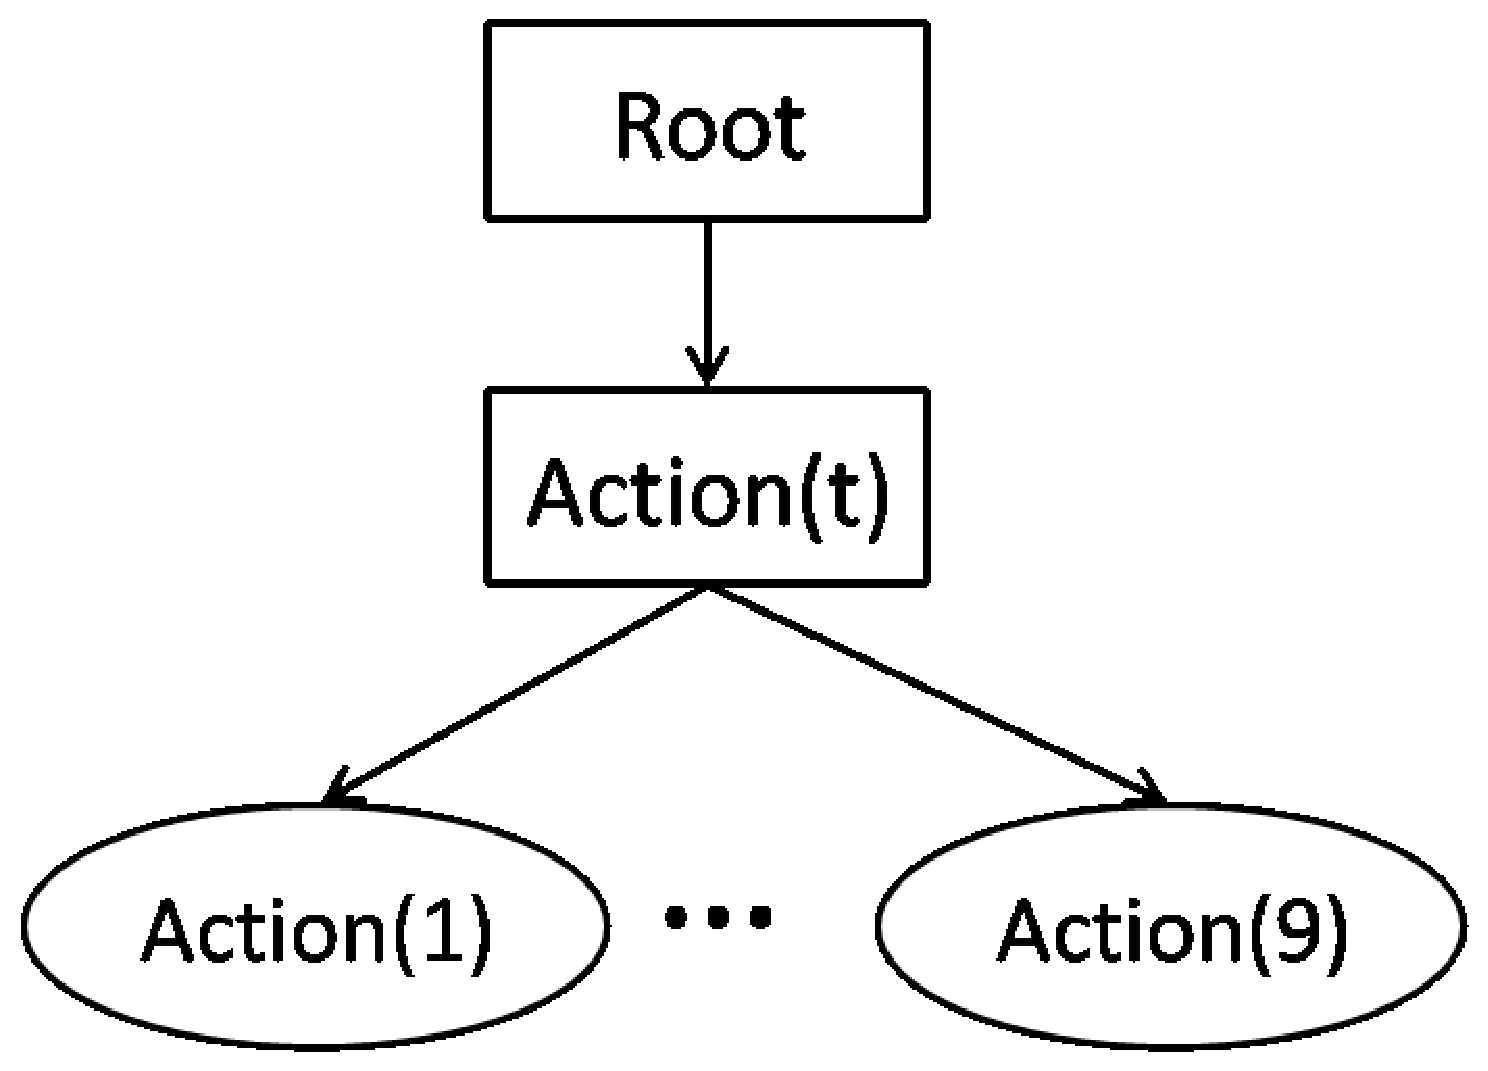
\includegraphics[width=3.0in] {./figures/MarioHierarchy.eps}
    \end{center}
%\end{minipage}
%\begin{minipage}[b]{0.5\linewidth} \centering (a) \end{minipage}
%\begin{minipage}[b]{0.5\linewidth} \centering (b) \end{minipage}

\caption{A task hierarchy for Infinite Mario}
\label{fig:MarioHierarchy}
\end{figure}
We combine the model-based method and model-free method with the task hierarchy shown in Fig. \ref{fig:MarioHierarchy}.
The model-based method is responsible for subtask $Root$ and the model-free method is for
subtask $Action(t)$.
For each step, subtask $Root$ selects one of the actions to execute.
Subtask $Action(t)$ then decide if it is going to follow the action suggested by $Root$ or not. 
If it does, $Action(t)$ will receive a pseudo-reward. 
Since $Action(t)$ is the only subtask that executes the primitive action,
the behaviour of the agent solely depends on its decision.
Subtask $Root$ can only influence its decision with the pseudo-reward.
Note that $Action(t)$ will terminate immediately after executing a single primitive action.
There is no temporal and spatial abstraction in this hierarchy.
That means that we do not enjoy any benefits from adopting the HRL framework.
In fact, the reason we adopted the HRL framework is to combine different methods.
And the benefit of doing so does not come from the HRL framework, but from the power of combining
model-free and model-based methods.

Unlike our approach with the Bus domain, we do not have 
individual subtask $Action(t)$ defined for each primitive action. 
Since subtask $Action(t)$ knows that it will be rewarded if it follows 
the action of $Root$, there is no need for us to separately learn the Q-function for every possible action. 
Instead, we use a single subtask $Action(t)$ to learn the Q-function for the original MDP. 
And the decision of $Action(t)$ is biased with the pseudo-reward when it is going to select the best action to execute. 
Thus, the method presented here does not have the overhead of maintaining multiple Q-functions as in our method for Bus domain.
%For this hierarchy, there is one 

%The state transition function and reward function depend on the policy of 
%child subtask, because the child subtask invoked by $root$ may not correspond to the primitive action that is executed by Mario.
%It would be more difficult if the effects and the policy are learned at the same time. 
%Instead, the transition function is learned from the primitive action that is executed by Mario.

For this special hierarchy, the pseudo-reward imposes a very interesting property:
the policy is identical to the policy of model-free method when a pseudo-reward is equal to zero and
it is identical to the one of model-based method given a sufficiently large pseudo-reward.
We can adjust the value of pseudo-reward to alternate the agent's behaviour between
two different methods.


\subsection{The result of Infinite Mario}
\label{se:MarioRes}
\begin{figure}[t]
 \begin{minipage}[b]{1.0\linewidth}
    \begin{center}
    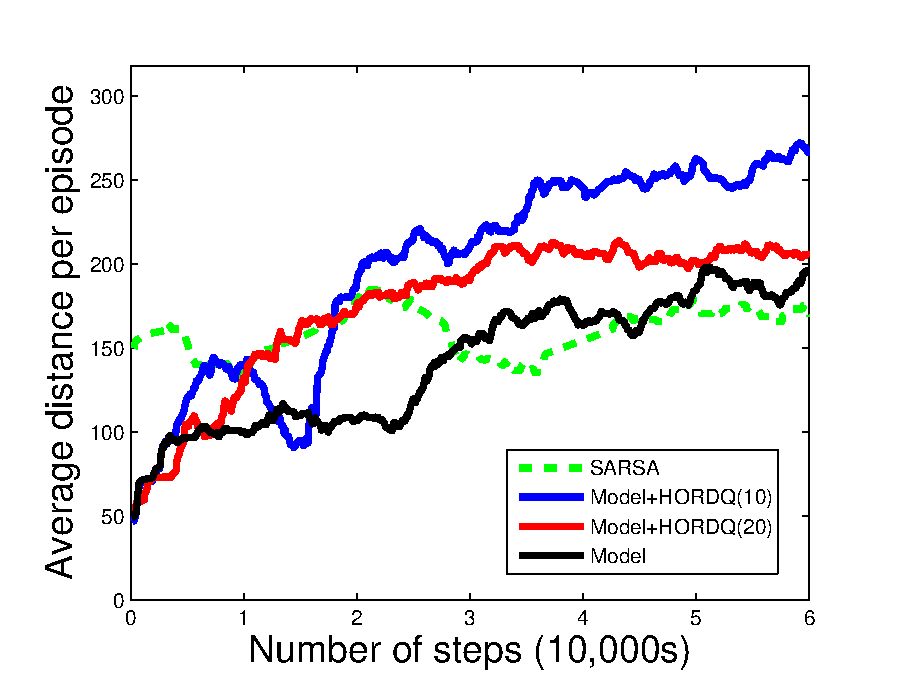
\includegraphics[width=4.0in] {./figures/1247.eps}
\end{center}
\end{minipage}

\caption{The distance that Mario moves for each episode, averaged over 20 episodes.
The parameters are $\alpha=0.05$ and $\gamma=0.7$. The exploration policy
$\epsilon$-greedy with $\epsilon = 0.01$.}
\label{fig:MarioExp}
\end{figure}


\begin{table}
    \begin{center}
\begin{tabular}[h]{l|l}
%\hline
%\multicolumn{1}{c}{}\\
\hline
Method Name & \# of finishing a level\\
\hline
SARSA    & 1\\
Model+HORDQ(10)    & 277\\
Model+HORDQ(20)     & 64\\
Model        & 0\\
\hline
\hline
\end{tabular}
\end{center}
\caption{The number of times for Mario to finish the level within 1000 runs}
%\caption{The features used by predicates.}
\end{table}

%The exploration policy in model-free approach is enough to let Mario explore the 
%unknown actions. It is not necessary for model-based approach to have the exploration policy as well. 
%XX is a special hierarchy. It allows us to combine two different methods under the HRL
%framework even for a problem without clear hierarchical structure. 
%no overhead

The level is generated with Infinite Mario simulator of RL competition 2009. The random seed is 1247
with type 0 and the difficulty is 3.
The maximum distance for Mario to move to the right is 315.
Beyond that, the level is finished with +100 reward.

%Bruno when random seed 1247, are you talking about a specific run? If so, what's special about this one in specific? Is it typical of something?
%James No, it is not typical. It is just a random trial.

Table 1 shows the number of times for Mario to finish the level within 1000 episodes.
Unsurprisingly, the model-based and model-free method are difficult
to finish a level because they may fail to handle either monsters or pits.
The model-based method only includes the dynamics of Mario, and ignores the rest of effects in game.
Thus, the learned policy can get Mario killed. On the other hand, the features of model-free method
do not include the information of pits, so it may fall into a pit.

Figure \ref{fig:MarioExp} shows the distance travelled by Mario with different pseudo-rewards.
Unlike the experiment in the Bus domain, the model-based method does not have
a better learning rate then the model-free method. The problem is that the model-based method
may lead Mario to be killed by a monster in an early state, thus it suffers a decreased learning rate.

If we combine both methods, we can see that Mario now can learn a better policy since
it can avoid both pits and monsters.
If we increase the pseudo-reward, the chances for Mario to be killed will increase, as it follows
the action of model-based method more often.
If we decrease the pseudo-reward, the chances to fall into a pit will increase, as the model-free  
method ignores the pit completely.

Our approach actually suggests a way to mix different methods and learn a better policy.
\ \\
\ \\
\ \\
\ \\
\ \\
\ \\
\ \\
\ \\
\ \\
\ \\
\ \\
\ \\
\ \\
\ \\
\ \\
\ \\
\ \\
\ \\
\ \\
\ \\
\ \\
\ \\
\ \\
\ \\
\ \\
\ \\
\ \\
\ \\
\ \\
\ \\
\ \\
\ \\
\ \\
\ \\
\ \\
\ \\
\ \\
\ \\
\ \\
\ \\
\ \\
\ \\
\ \\
\ \\
\ \\
\ \\
\ \\
\ \\
\ \\
\ \\
\ \\
\ \\
\ \\
\ \\
\ \\
\ \\
\ \\
\ \\
\ \\
\ \\
\ \\
%From experiment, 
\endinput
%Most of the previous work on RL focus on model-free approaches for several reasons. 
%The most 
%Within a planning agent, there are at least two roles for real experience: it
%can be used to improve the model (to make it more accurately match the real
%environment) and it can be used to directly improve the value function and
%policy using the kinds of reinforcement learning methods we have discussed in
%previous chapters. The former we call model-learning, and the latter we call
%direct reinforcement learning (direct RL). The possible relationships between
%experience, model, values, and policy are summarized in Figure  9.2. Each arrow
%shows a relationship of influence and presumed improvement. Note how experience
%can improve value and policy functions either directly or indirectly via the
%model. It is the latter, which is sometimes called indirect reinforcement
%learning, that is involved in planning. 

%The second branch is model-based RL, which directly estimates
%a model of the environment and then plans with
%this model. Early work demonstrated that summarizing an
%agent’s experience into a model could be an efficient way
%to reuse data (Moore & Atkeson, 1993), and later work utilized
%the uncertainty in an agent’s model to guide exploration,
%yielding the first (probabilistic) finite bounds on the amount of data required
%to learn near-optimal behaviors in the general case (Kearns & Singh, 1998;
%Kakade, 2003).


%motivation: play a randomly generate maze to adapt to
%adapt to noval situation

%weakness-> an adversary to block the path forever
%no knowledge (coin won't disappear-->need hack to do it, moster won't move)
%comparison to the previous work->HRL,


%model based-> state space is too large. good to train with
%few examples (10 sec training)
%model free-> cannot handle randomly generated maze -> failed to adapt to noval situation. can handle large space (linear SARSA)
%Experiment: comparison with flat model based approach and hierarchical model based approach with approximation

%combine both-> use model based on top level to reduce
%the state space, and model free on bottom to 
%deal with randomized noisy world for short term reward

%build multilevel of hierachy on features
%label each room with a number 1, 2, 3
%the coordinate of wrt the room
%(1, (25, 30))
%move from room 1 to room 2
%top level
%action (1->2)
%second level
%assume (1, (25, 30)) -> (2, (0, 0))
%action ((25, 30) -> (0, 0)) goal (-25, -30) in single step

%need to build time model of the full state
%P(s->s'|x, t) the propability to move from state s to s'
%after t steps of the observation of full state x

%power coms from trasition model (model the shortest path), not shortest path
%you can use model-based approach on this

%fickle passenger of MaxQ
%coarseness on time and space scale

%-->you can work on continus varible now, no more grid world

%1. Assumption on the state difference (if it is not true --> like the agent in a world boundary or the health is 100 and cannot be imporve
  %since the state is outside the known state boundary, the planner whon't plan for it. but the local planner may still direct the agent
  %to go outside the world boundary, which may be a problem)
%2. Application to the hierachical RL
%3. Limitation: unachievable state (a coin surrounded by many monsters)
%4. Can inference in a very small world, not need to do 64 by 64
%Sometimes we need a plan. The greedy approach of reinforcement learning does not always work. 
%RL techniques have several limitations:
%1. It's difficult for to transfer the value function from a small world to a large one. If the agent has
%the experience only in a small world like 4 \times 4 grid, it cannot act well in 64 \times 64 grid
%because it does not know the correct action in regard to an object 63 grid away.

%2. It takes a long time to train the agent to be good enough. The greedy 

%3. The approximation only good in a small range. We need a plan for long term action.
%The noval state (the state in current game which has not been experienced) may 

%4. Impossible task to maze problems: RL require that optimal agent to find the optimal solution for a maze when all the features
%are input to the agent. Which is unlikely to work.(impractical when the maze is large)(unable to transfer
%the knowledge from previous maze experience to the current one) A practical solver shall invovle planning through 
%the possible route and find the one which can lead to the exist.
%All the work requires the agent to repeat play the same maze (assuming traps) until it finds the optimal solution.
%What if the maze changes every time?

%1. Is it guarranteed convergence? Yes, if we choose the goal next to the current state which leads to highest Q value. 
%It is the same as SARSA.
%2. How to choose the goal to guarrante convergence to optimal policy?

%Good to work on the problem with a long term reinforcement (feedback) like a maze.
%Bad to work with a problem with dynamic envirment (everything changes with or without agents actions)
%Bad when the consequence of an action is delayed for many steps. (poison)

%Q: prove that RL cannot solve maze problem
%Ability to transfer the knowledge from one maze to another
%compare the HRL in key-finding problem
%compare to the model-based RL





%application: the key-room problem--> each room lock a key, one room has a treasure, the agent needs to go through 
%a maze to collect the keys for each door and get the treasure

%Stochastic Shortest-Path Problems
%A Stochastic Shortest-Path problem is an mdp prob-
%lem in which the state space S = f1; : : : ; n; tg is such
%that t is a goal (target) state that is absorbing (i.e.,
%p(t; u; t) = 1 and g(t; u) = 0 for all u 2 U(t)), and the
%discount factor ® = 1. In this case, the existence of
%optimal policies (and optimal stationary policies) is a
%major mathematical problem. However, the existence
%is guarantee under the following reasonable conditions:
%(A1) There exists a policy that achieves the goal with
%probability 1 from any starting state.
%(A2) All costs are positive.
%The ¯rst assumption just expresses the fact that the
%problem admits a well-behaved solution. Such policies
%are known as proper policies. The second assumption,
%in the other hand, guarantees that all improper policies
%incurs in in¯nite cost for at least one state. Thus, both
%assumptions preclude cases where the optimal solution
%might \wander" around without never getting to the
%goal. For example, a problem having a zero-cost cycle
%(in state space) violates the second assumption.
%As mentioned in the Introduction, often we are only
%interested in knowing how to go from a ¯xed initial
%state, say 1, to the goal state. The optimal solution in
%this case is an partial optimal stationary policy ¹ such
%that ¹(i) = ¹¤(i) for all states i that are reachable
%from 1 when using the optimal policy ¹¤; the so-called
%relevant states when starting from 1.1
%Finding a partial optimal policy can be consider-
%ably simpler, the extreme case when the set of relevant
%states is ¯nite and the complete state space is in¯nite.
%Thus, the question of how to ¯nd partial optimal poli-
%cies is of great relevance. One algorithm for that is
%Real-Time Dynamic Programming.

%There are two ways for a RL agent to use its sample data. It can use the sample data to update the 
%value function and improve its policy. It is called model-free (or direct) reinforcement learning. 
%Another approach is to use the sample data to estimate parameters for the model of the environment and compute the value function
%from the model. It is called model-based (indirect) reinforcement learning.

%The advantage of model-based approaches is that they make more efficient use of the sample data, thus 
%it take fewer time to train a model-based RL agent. Other the other hand, model-free approaches do not assume 
%a prior model, so it would not be affected by the bias of the model design. Besides, the existence of 
%good linear approximation algorithms, such as linear SARSA, makes it possible for model-free approaches to
%handle large scale problems.

%Model-based approaches needs to enumerate through all possible states to compute the value function. 
%But the number of states grows exponentially with the number of features, 
%and it quickly becomes intractable if the number features grows large.

%The main idea of this work is to combine the model-free, model-based and hierarchical reinforcement learning.
%For the lower level of hierarchy, we adopt the model-free approach to handle the complete and possibly large state space.
%On the top level of hierarchy, we use the model-based to plan on a coarser level, which contains only small number of states.
%This approach allows the agent to plan on the higher level and make efficient use of the sample data. On the lower level,
%the agent uses model-free approaches with linear approximation to handle the complete state space.

%The prior works on hierarchical reinforcement learning (HRL) can be divided into two categories: model-free and model-based approaches. 
%The model-free approaches include HAMQ \cite{HAMQ}, MAXQ \cite{MAXQ}, SMDP and options framework \cite{option}
%For model-based approaches, Seri et al. \cite{HLearning} proposed a model-based HRL in average reward setting.
%Diuk et al. \cite{Diuk} adopted model-based HRL to deterministic domain. Jong and Stone \cite{RMaxQ} combined 
%R-MAXQ and MAXQ to achieve efficient model-based exploration and the action abstraction of MAXQ.

%TODO: show that model based state difference can learn randomly generated maze with very limited steps (only four touches of the wall)
%TODO: use a poison example to show the limit of pure approximated model-based approach and the motivation
%of use hierarchical optimal policy for pseudo reward and recursive optimal policy for real reward. It can be shown that
%it will converge to optimal policy if the true goal state of the game is included as a subgoal(
%the worst case is the child node finish the game by itself)
